
\chapter{Industrielle roboter}

Dette kapittelet består foreløpig i notatform. 
$$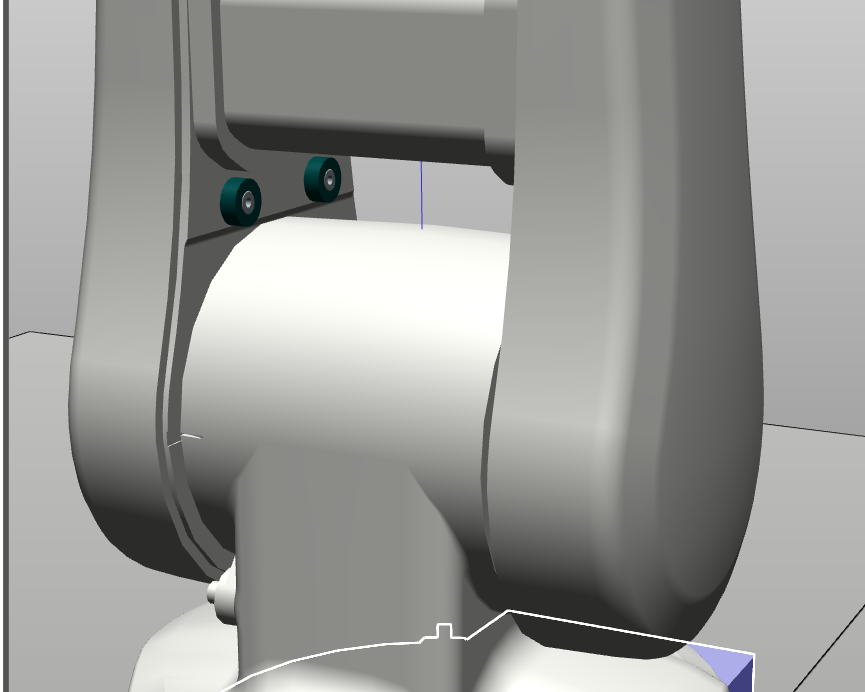
\includegraphics[width=16cm]{./Robot01.png}$$
\section{trandisjonelle roboter}

Insustrielle roboer har ofte en struktur som en mennesklig arm.

\begin{itemize}%%[noitemsep]
\item opp til  6 akser
\item plukk og plaser syklus på 300-500ms med deler på et par kg. 
\item Sveiseroboter
\end{itemize}


Hva kjennetegner en industriell robot:
\begin{itemize}%[noitemsep]
\item den kjører automatisk
\item den kan reprogrammeres
\item den har en arm med mer en tre akser som en kan feste ulike verktøy på
\item den kan enten stå fast eller være flyttbare
\item den er laget for å løse industrelle oppgaver 
\end{itemize}

Ulike industrielle roboter kan være:
\begin{itemize}%[noitemsep]
\item Linære roboter
\item SCARA roboter
\item Parallelle roboter
\item Artikulerte roboter
\item Sylindriske roboter
\end{itemize}

Eksempler på industrielle bruksområder:


\begin{itemize}%[noitemsep]
\item Forflytting av metall i deleproduksjon eller støyping
\item palletering
\item sveising
\item lakkering
\item pakking
\item automatisk lagersystem
\end{itemize}



Mekanisk teori:
\begin{itemize}%[noitemsep]
\item mekanismer og grader av frihet
\item kinematikk?
\item Arbeidsområde og leddområde
\item redundans og singularitet
\end{itemize}

Styring:
\begin{itemize}%[noitemsep]
\item bane planlegging
\item posisjon, kraft og impedanse kontrol
\item læring av baner
\end{itemize}



Robotsystemer:
\begin{itemize}%[noitemsep]
\item Robots functional schematics
\item End-effectors and tools
\end{itemize}







%%%%%%%%%%%%%%%%%%%%%%%%%%%%%%%%%%%%%%%%%%%%%%%%%%%%

